%
% 2-Applications.tex
%
%  LaTeX source file for section 2 Applications for the Conceptual Clustering lab module of the TAILS project.
%

\section{Applications}
Conceptual clustering is widely used in our life. Learning itself is a kind of conceptual clustering. As a child grows up, he may learn to play toy blocks, count, recognize shapes and letters, he may learn maths, drawing, reading and writing, and later he may learn Artificial Intelligence, arts and English literature. Each time when a child learns something new, new knowledge will be stored in his knowledge base and relate to what he has already known or span a new space in his knowledge base. Similar knowledge is grouped together to form a category. As time goes by, the knowledge base broadens just like the classification tree spans. For example, when a student learns geometry in middle school, he may automatically add his previous experience with shapes to the new subject. Later when he learns architecture in college, he may probably reorganize his knowledge by adding geometry as the child node of architecture. Reference to Figure\ref{Fig:app1}. Those knowledge categories in mind help a person to respond to the problems from the outside world smoothly. For example, when the student participates a group project about designing a museum, he may need to search the related knowledge category in mind like architecture, recall related experience and finally reacts to the problem.

\begin{figure}[h!]
    \centering
    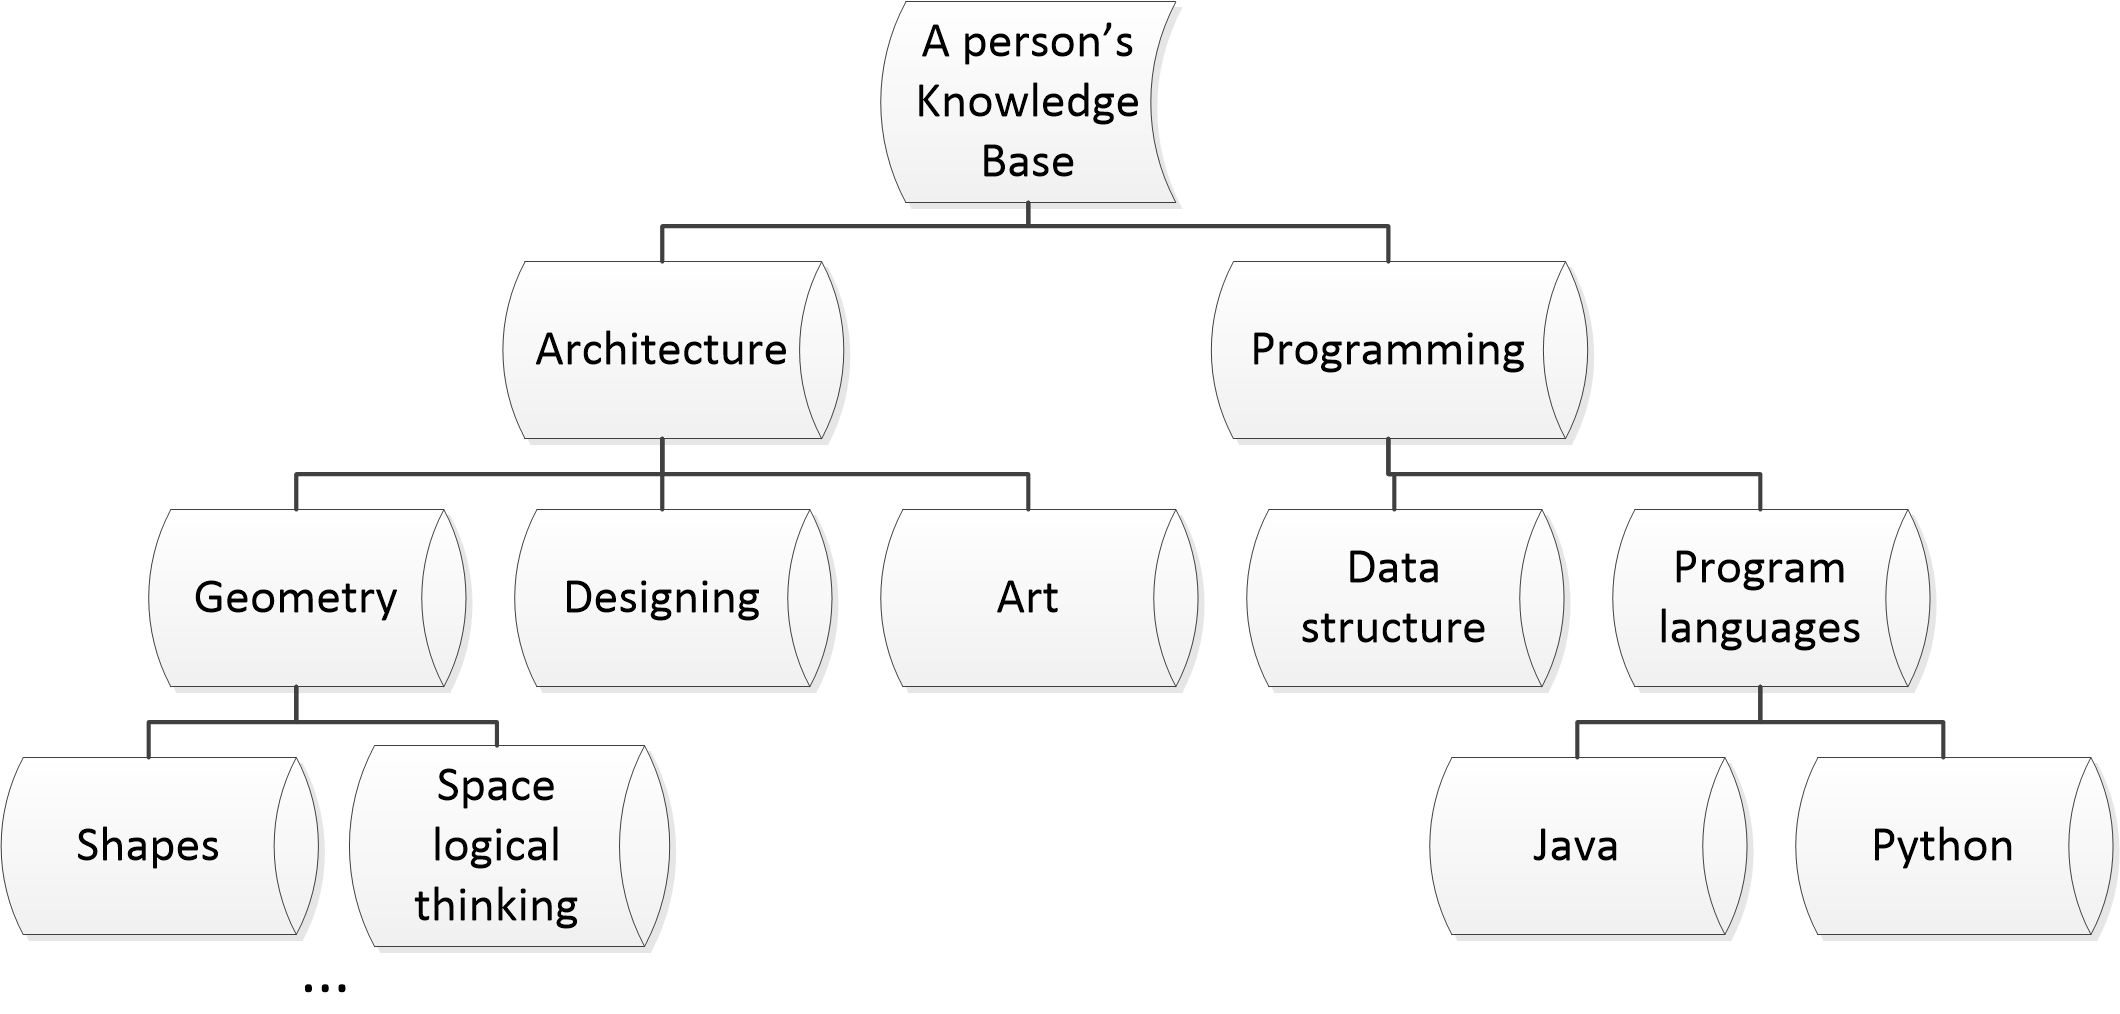
\includegraphics[width=300pt]{../images/app1.jpg}
    \caption{An example of classification tree for a person's knowledge base}
    \label{Fig:app1}
	\end{figure}
	
Another possible example is that zoologist finds some new species from a isolated island. He may need to examine the new species from the structure or gene to decide if the new species belongs to any known class or it is a new class. The classification tree is shown in Figure \ref{Fig:app2}
\begin{figure}[h!]
    \centering
    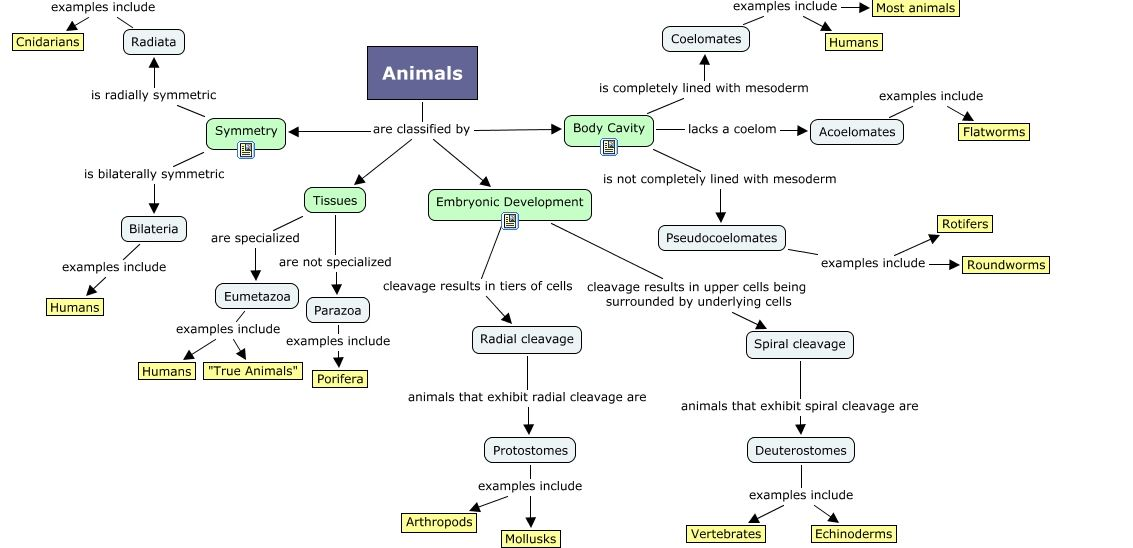
\includegraphics[width=400pt]{../images/app2.jpg}
    \caption{The classification tree for animals\cite{newyork}}
    \label{Fig:app2}
	\end{figure}


